% Gravity network---graphical exposition of migration flows in a gravity network
% Author: Thomas de Graaff
\documentclass{standalone} 
\usepackage{tikz, verbatim}
\usepackage{pgfplots}   %include other needed packages here    
%\usepackage[active,tightpage]{preview}
\usetikzlibrary{shapes, backgrounds}
%\PreviewEnvironment{tikzpicture}
%\setlength\PreviewBorder{0pt}%
\begin{comment}
:Title: Gravity network---graphical exposition of migration flows in a gravity network
:Tags: pgfplots, migration, gravity
:Author: Thomas de Graaff

This plot describes the flows from origins to destinations and the various variables that can be used to describe the impact of both origins and destination and the variables that measure the impacts of "distance".
\end{comment}
\begin{document}   

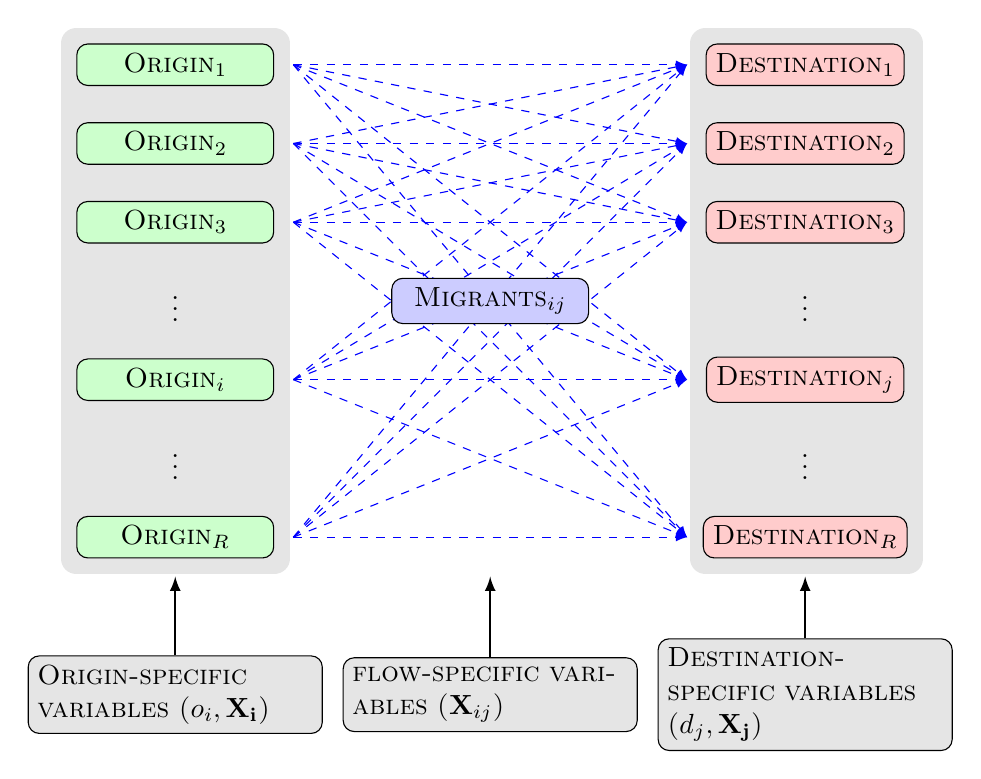
\begin{tikzpicture}[scale=1,thick]

\tikzstyle{orig}=[rectangle, rounded corners, thin, fill=green!20, text=black, draw, minimum width=2.5cm]
\tikzstyle{dest}=[rectangle, rounded corners, thin, fill=red!20, text=black, draw, minimum width=2.5cm]
\tikzstyle{migrants}=[rectangle, rounded corners, thin, fill=blue!20, text=black, draw, minimum width=2.5cm]
\tikzstyle{var}=[rectangle, rounded corners, thin, fill=black!10, text=black, draw, text width = 3.5cm]

  	\node[orig] (o1) at (0,0)  {\textsc{Origin$_1$}};
	\node[orig] (o2) at (0,-1) {\textsc{Origin$_2$}};
	\node[orig] (o3) at (0,-2) {\textsc{Origin$_3$}};
	\node (o4) at (0,-3) {\textsc{\vdots}};
	\node[orig] (o5) at (0,-4) {\textsc{Origin$_i$}};
	\node (o6) at (0,-5) {\textsc{\vdots}};
	\node[orig] (o7) at (0,-6) {\textsc{Origin$_R$}};
	
  	\node[dest] (d1) at (8,0)  {\textsc{Destination$_1$}};
	\node[dest] (d2) at (8,-1) {\textsc{Destination$_2$}};
	\node[dest] (d3) at (8,-2) {\textsc{Destination$_3$}};
	\node (d4) 		 at (8,-3) {\textsc{\vdots}};
	\node[dest] (d5) at (8,-4) {\textsc{Destination$_j$}};
	\node (d6) 		 at (8,-5) {\textsc{\vdots}};
	\node[dest] (d7) at (8,-6) {\textsc{Destination$_R$}};
	
	 % Migratior links
  	\draw[-latex, blue, thin, dashed] (1.5,0) -- (6.5, 0);
	\draw[-latex, blue, thin, dashed] (1.5,0) -- (6.5,-1);
	\draw[-latex, blue, thin, dashed] (1.5,0) -- (6.5,-2);
	\draw[-latex, blue, thin, dashed] (1.5,0) -- (6.5,-4);
	\draw[-latex, blue, thin, dashed] (1.5,0) -- (6.5,-6);
	
	\draw[-latex, blue, thin, dashed] (1.5,-1) -- (6.5, 0);
	\draw[-latex, blue, thin, dashed] (1.5,-1) -- (6.5,-1);
	\draw[-latex, blue, thin, dashed] (1.5,-1) -- (6.5,-2);
	\draw[-latex, blue, thin, dashed] (1.5,-1) -- (6.5,-4);
	\draw[-latex, blue, thin, dashed] (1.5,-1) -- (6.5,-6);
	
	\draw[-latex, blue, thin, dashed] (1.5,-2) -- (6.5, 0);
	\draw[-latex, blue, thin, dashed] (1.5,-2) -- (6.5,-1);
	\draw[-latex, blue, thin, dashed] (1.5,-2) -- (6.5,-2);
	\draw[-latex, blue, thin, dashed] (1.5,-2) -- (6.5,-4);
	\draw[-latex, blue, thin, dashed] (1.5,-2) -- (6.5,-6);
	
	\draw[-latex, blue, thin, dashed] (1.5,-4) -- (6.5, 0);
	\draw[-latex, blue, thin, dashed] (1.5,-4) -- (6.5,-1);
	\draw[-latex, blue, thin, dashed] (1.5,-4) -- (6.5,-2);
	\draw[-latex, blue, thin, dashed] (1.5,-4) -- (6.5,-4);
	\draw[-latex, blue, thin, dashed] (1.5,-4) -- (6.5,-6);
	
	\draw[-latex, blue, thin, dashed] (1.5,-6) -- (6.5, 0);
	\draw[-latex, blue, thin, dashed] (1.5,-6) -- (6.5,-1);
	\draw[-latex, blue, thin, dashed] (1.5,-6) -- (6.5,-2);
	\draw[-latex, blue, thin, dashed] (1.5,-6) -- (6.5,-4);
	\draw[-latex, blue, thin, dashed] (1.5,-6) -- (6.5,-6);
	
	\node[migrants] (m) at (4,-3)  {\textsc{Migrants$_{ij}$}};
	
	\node[var] (v1) at (0,-8)  {\textsc{Origin-specific variables ($o_i, \mathbf{X_i}$)}};
	\node[var] (v2) at (4,-8)  {\textsc{flow-specific variables ($\mathbf{X}_{ij}$) }};
	\node[var] (v3) at (8,-8)  {\textsc{Destination-specific variables  ($d_j, \mathbf{X_j}$)}};
	
	\begin{pgfonlayer}{background}
		\filldraw [line width=4mm,join=round,black!10]
			(o1.north -| o1.west)  rectangle (o7.south -| o7.east)
			(d1.north -| d1.west)  rectangle (d7.south -| d7.east);
	\end{pgfonlayer}
	
    \draw[-latex, thick, black] (v1) -- (0,-6.5);
	\draw[-latex, thick, black] (v2) -- (4,-6.5);
	\draw[-latex, thick, black] (v3) -- (8,-6.5);
\end{tikzpicture}
\end{document} 